\chapter{Camera}
\section{Camera pipeline}
Si possono riconoscere due principali tipologie di camere:
\begin{itemize}
    \item \textbf{mobile}: camera dei cellulari con sensore piccolo, ottica fissa 
    e zoom limitato, ma ha un basso costo e un'alta potenza di calcolo.
    \item \textbf{digital single reflex camera}: sensore più grande con ottica mobile 
    e zoom ottico, ma ha un alto costo e ridotta potenza di calcolo.
\end{itemize}

In aggiunta possiamo avere camere meno professionali che sono una via di mezzo 
tra le reflex e quelle degli smartphone.

La pipeline di elaborazione delle reflex è la seguente:
\begin{itemize}
    \item acquisizione dell'immagine
    \item grezzo bilanciamento del bianco
    \item compressione lossless
    \item formattazione dei metadati
    \item salvataggio
    \item decompressione
    \item color-sensor denoising
    \item bilanciamento del bianco
    \item processamento del colore
\end{itemize}

La pipeline di elaborazione delle camere consumer è la seguente:
\begin{itemize}
    \item acquisizione dell'immagine
    \item color-sensor denoising
    \item bilanciamento del bianco
    \item colorcorrection
    \item tone scale rendering
    \item sharpening and noise reduction
    \item jpeg compression
    \item formattazione dei metadati
    \item salvataggio
\end{itemize}

La pipeline di elaborazione delle camere degli smartphone \textbf{single frame} si 
suddivide in due regioni:
\begin{itemize}
    \item \textbf{raw processing}: 
    \begin{itemize}
        \item raw image preprocessing
        \item bayer denoising
        \item white balancing
        \item color space convertion from DD to DI
    \end{itemize}
    \item \textbf{image processing (enhancement)}: 
    \begin{itemize}
        \item color manipulation
        \item tone mapping
        \item noise reduction
        \item sharpening
        \item output color shape convertion in DD
        \item image resizing
        \item jpeg compression
        \item saving
    \end{itemize}
\end{itemize}

La pipeline di elaborazione delle camere degli smartphone \textbf{multi frame} si 
suddivide in due regioni:
\begin{itemize}
    \item \textbf{raw processing}: 
    \begin{itemize}
        \item raw image preprocessing
        \item multiframe alignment
        \item multiframe merge
        \item white balance
        \item color space convertion from DD to DI
    \end{itemize}
    \item \textbf{image processing (enhancement)}: 
    \begin{itemize}
        \item color manipulation
        \item tone mapping
        \item image processing enhancement
        \item saving
    \end{itemize}
\end{itemize}

In generale per effettuare il processing delle immagini si utilizzano dei chip
hw che vengono programmati dalle aziende.

\section{Modello della camera}
Le camere si basano sul modello della pin hole camera e sulla proiezione prospettica 
(vedi appunti CV).

Un componente importante è la velocità dell'otturatore che più è alta allora più 
avremo effetti di motion blur e più è bassa e meno motion blur si avrà in scene 
dinamiche.

Per catturare delle immagini colorate ci sono diversi metodi:
\begin{itemize}
    \item \textbf{Field sequential}: unico sensore con un cilidro con $3$ filtri (R, G, B),
    si scattano $3$ immagini sequenziali ciascuna con un filtro diverso e poi si 
    compongono per ottenere l'immagine risultante. Si hanno problemi con scene 
    dinamiche perché avremo $3$ frame differenti.
    \item \textbf{Multi-chip}: si utilizzano $3$ sensori diversi uno per ogni colore e un 
    prisma che separa le frequenze e le ridirige sui singoli sensori. Risolve i
    problemi di quello precedente, aumenta il costo ed è meno robusto perché se si 
    disallineano il prisma e i sensori si hanno immagini con peggior qualità.
    \item \textbf{Bayer filter}: si utilizza un unico sensore, si piazzano i filtri 
    colore su ciascun pixel creando diversi pattern. Si hanno quindi $3$ immagini 
    di risoluzione diversa, si combinano interpolando i colori vicini.
    \item \textbf{x3 technology} (stacked sensor): si hanno $3$ strati di silicio diferenti 
    posizionati uno sopra all'altro su ogni pixel del sensore, ciascuno assorbe solo una frequenza
    e in questo modo si ottiene un image per ciascun canale ma della stessa risoluzione.
\end{itemize}

Si hanno poi $2$ tipologie di sensori:
\begin{itemize}
    \item \textbf{CCD} (charge coupled device): muove l'immagine tra i pixel per 
    convertirla in corrente fuori dal sensore. Tecnologia più matura perché si ha 
    maggior sensibilità, HDR, low-noise image, si ha maggior densità dei pixel, ma 
    consuma di più.
    \item \textbf{CMOS} (complementary metal oxide semiconductor): converte l'energia dell'elemento sensibile direttamente 
    in corrente sul pixel. Questo implica che si possono applicare direttamente dei 
    processing sul pixel inplace, necessita di meno corrente, meno sensitivo, più
    comodo per lo standard silicon production ed è più veloce di CCD.
\end{itemize}

Scattando foto con le camere possiamo trovare degli artefatti legati alla sovraesposizione 
dei singoli pixel e al rumore:
\begin{itemize}
    \item \textbf{bloom}: quando un pixel arriva a saturazione trasmette energia 
    anche ai pixel vicini (CMOS e CCD).
    \item \textbf{smearing}: stessa cosa ma trasmette ai pixel sulla colonna (CCD 
    perché i pixel sulla colonna sono più vicini)
\end{itemize}

La qualità dell'immagine del sensore dipende principalmente da quanta luce viene 
assorbita dai singoli pixel del sensore, per aumentare la luce spesso si utilizzano 
delle \textbf{microlenti} sul singolo pixel per ridirezionare la luce dentro al pixel.

In aggiunta, più un sensore è grande e più è resistente al rumore, mentre a parità 
di dimensione tra due sensori, se uno ha più pixel allora sarà soggetto a rumore, 
al contrario se uno ha meno pixel sarà soggetto a meno rumore e quindi sarà migliore.

I singoli pixel sensibili alla luce hanno una relazione pseudo lineare di conversione 
fotoni-elettroni. In realtà sarà non lineare a causa del rumore quando si hanno 
pochi fotoni, al contrario sarà non lineare quando raggiungiamo la saturazione del
pixel.

Il rumore presente nelle camere è di due tipologie:
\begin{itemize}
    \item \textbf{optional crosstalk}: si hanno fotoni filtrati dal pixel adiacente ma 
    entra nel pixel accanto che ha un altro filtro colore
    \item \textbf{electrical crosstalk}: alcuni fotoni vengono irradiati verso i pixel 
    vicini
\end{itemize}

Nota che il sensore può percepire le frequenze NIR, per renderlo più simile a allo 
spettro di assorbimento dell'occhio umano si applica un filtro delle frequenze NIR 
su tutto il sensore.

Per ridure il rumore  dei pixel e migliorare le immagini buie Kodak ha creato un Bayer filter con dei filtri bianchi
che permettono di incrementare la luce entrante e ridurre il rumore e ridurre la 
dimensione del sensore. Il problema è
richiede algoritmi di interpolazione più complessi e correggere gli errori è più
complesso.

Per ridurre il rumore sempre in Bauer filter si possono applicare dei filtri colori 
uguali su più pixel adiacenti: 2x2 o 3x3. In questo modo si possono aumentare il 
numero di pixel.

Possiamo avere molti problemi durante l'acquisizione dell'immagine:
\begin{itemize}
    \item \textbf{vignetting e pixel non uniformi}: illuminazione non uniforme sul frame, questo si 
    può risolvere fotografando un muro bianco e invertendo la maschera otteniamo 
    la maschera del rumore che possiamo aggiungere all'immagine per eliminare l'effetto.
    Un'altra soluzione è quella di utilizzare un sensore più piccolo e centrato nell'
    asse ottico.
    \item \textbf{defective pixel}: possiamo avere dei pixel bruciati sul sensore
    e quindi si hanno o pixel nulli o pixel con massima saturazione. Per risolvere 
    questo problema basta scattare una foto della scena al buio, otteniamo i pixel 
    dead, poi effettuiamo un'interpolazione dei pixel. 
    \item \textbf{dark floor}: generalmente si sacrifica la cornice del sensore per 
    stimare il rumore, in questo modo una volta stimato possiamo correggerlo.
    \item \textbf{distorsioni}: con l'utilizzo delle lenti possiamo avere delle
    distorsioni del frame, per correggerle possiamo effettuare una foto ad un muro 
    con delle linee che si intersecano, successivamente applichiamo delle trasformazioni
    per riportare le linee parallele ed equidistanti. 
\end{itemize}

\subsection{ISO block}
Il primo passo della pipeline è quello di convertire un segnale analogico in digitale,
durante questa conversione si può avere un'amplificazione del segnale che nelle macchine 
si specifica con ISO. Questa amplificazione permette di migliorare la visibilità
dell'immagine quando c'è tanta luce o poca, il problema che aumenta anche il rumore
e satura più velocemente il sensore. Per risolvere questi problemi dobbiamo cambiare 
l'apertura o la velocità dell'otturatore.

Sapendo che l'essere umano ha una gamma correction non lineare, allora si applica la 
stessa cosa anche alle immagini in fase di digitalizzazione. Più precisamente si campiona 
il segnale in modo non uniforme rispetto al suo valore, ma si capiona in modo uniforme rispetto
alla percezione. 

\begin{nota}
    Quando applichiamo la gamma correction non lineare in fase di acquisizione, se
    dobbiamo mostrare a schermo un'immagine allora si riapplica una gamma correction 
    inversa per ottenere una linearità dei colori nell'immagine.
\end{nota}

Sempre in fase di acquisizione è importante specificare la velocità dell'otturatore
perché ci permette di avere effetti di motion blur.

\subsection{Image demosaicing}
Quando utilizziamo camere basate su Bayer filter dobbiamo interpolare i colori per 
ciascun pixel, questa operazione viene effettuata in questa sezione. Possiamo 
effettuare due interpolazioni:
\begin{itemize}
    \item linear interpolation: semplice ma pecca sui bordi
    \item linear interpolation + edge info: si effettua una linear interpolation intelligente 
    in base al gradiente in modo da non combinare colori che hanno una alta variazione.
\end{itemize}
\subsection{Noisy reduction}
Il rumore compare in fase di acquisizione, amplificazione e conversione da Analogico a Digitale.
Per ridurre il rumore si può utilizzare:
\begin{itemize}
    \item mean filtering: utile per un rumore gaussiano
    \item median filtering: utile per un rumore salt\&pepper
\end{itemize} 

Il rumore può essere più visibile in alcune regioni dell'immagine e meno visibile 
in altre, per esempio rispettivamente in regioni monocromatice e più dettagliate.
Possiamo quindi far variare l'intensità del denoising in base alle regioni utilizzando 
un texture detection.

\begin{figure}[h]
    \centering
    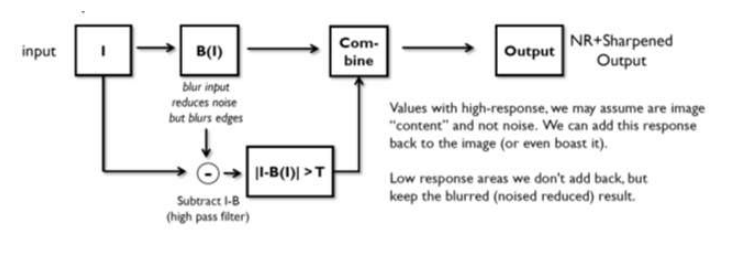
\includegraphics[width=0.5\textwidth]{img/denoising_gaussiano_adattivo.png}
    \caption{esempio di denoising adattivo sul gaussiano}
\end{figure}

\subsection{Automated correction}
La prima correzione automatica applicata è l'\textbf{autofocus} ed esistono diversi 
approcci:
\begin{itemize}
    \item \textbf{approcci attivi}: utilizzando gli infrarossi per calcolare la
    distanza del soggetto
    \item \textbf{passivi}: si analizza la frequenza spaziale dell'immagine per 
    stimare il focus come ad esempio il contrasto (più contrasto allora immagine a fuoco).
    Un esempio di autofocus è anche quello basato sugli edge e quindi usare il filtro 
    laplaciano.
    \item \textbf{smart}: si utilizzano i soggetti per mettere a fuoco, come le facce.
\end{itemize}

Abbiamo poi anche la selezione dell'\textbf{automated exposure}, ovvero la quantità 
di luce che entra e quindi il tempo di apertura dell'otturatore. In sostanza si 
effettua una media di intensità di alcuni pixel selezionati e utilizzare una soglia, esistono diverse maschere 
per selezionare i pixel. Possiamo anche basarci sulla skin-tone.

\begin{nota}
    PEr le camere HDR si effettuano multipli scatti e si effettua una combinazione
    delle immagini.
\end{nota}

Abbiamo anche l'\textbf{auto white balancing} si basa sulla stima del colore dell'illuminante 
della scena, per esempio sfruttando l'ipotesi di \textbf{grey world}. In sostanza 
si assume che un'immagine con una variazione di colori quando la continuiamo a sfocare 
arriveremo ad ottenere il colore grigio. Quando l'immagine non è bilanciata si ottiene 
il colore dell'illuminante e poi si applica la trasformazione. Il problema è che non 
otteniamo buoni risultati sempre. Possiamo migliorare escludendo i colori saturi,
considerando solo i pixel più illuminati.

\begin{nota}
    Prima avevamo visto il custom white balancing, ovvero quello supervisionato
    dove si utilizza una palette di reference o un oggetto bianco nella scena. La 
    versione automatica si basa sullo stimare l'illuminante e poi correggere.
\end{nota}

Un altro algoritmo di automatic white balancing è chiamato \textbf{max RGB} che 
si basa sulla referenza del bianco come il colore col max RGB nell'imamgine. Si basa 
sul ragionamento che il bianco rimane il massimo in ogni illuminante.

Un altro algoritmo di automatic white balancing è chiamato \textbf{white patch}
che sfrutta una superficie bianca nell'immagine per effettuare la regolazione.


\subsection{Post-processing}
Si applicano dei passi di post-processing per rendere le immagini più belle agli 
occhi dell'utilizzatore, le prime trasformazioni si basano sull'applicare una color 
correction in base alla regione geografica. In asia si tende a portare il colore della 
pelle verso il bianco.

Poi abbiamo \textbf{flare} ovvero un illuminante uniforme che crea una nebbia, si può
risolvere in due modi: il primo si sottrarre una percentuale della media dei pixel 
di tutta l'immagine, il secondo più adattivo è quello di sottrarre una percentuale 
fissa della media tra pixel vicini dell'immagine.

Poi abbiamo la gestione dei collori e del contrasto attraverso la gamma correction.

\subsection{Spazio colore standard del dispositivo}
I valori dei tristimoli variano tra dispositivo e l'altro, bisogna quindi convertire 
i colori dalle sensibilità allo standard sRGB.

\subsection{Compression}
Abbiamo poi la compressione jpeg applica andando a convertie in uno spazio colori 
che separa la luminanza e si comprime il colore non la luminanza.

\section{Filtering spatial domain}
Abbiamo visto i filtri mediani e gaussiani per rimuovere il rumore nelle immagini, 
il problema è che poi togliamo gli edge perché blurriamo. Possiamo usare un \textbf{non 
local means filter} che prende la media basata su altri intorni simili.

Un altro approccio è quello di usare il \textbf{bilateral filter} in sostanza permette 
di applicare filtri diversi in modo intelligente per rimuovere il rumore e preservare 
gli edge e le texture. Si basa sull'utilizzo di due parametri:
\begin{itemize}
    \item $\sigma_r$: regola l'applicazione sui pixel che hanno intensità simili 
    (regola l'ampiezza della gaussiana 1D)
    \item $\sigma_s$: regola l'ampiezza della gaussiana che regola la vicinanza spaziale.
\end{itemize}

Una volta applicato il bilateral possiamo calcolare il residuo e permette di trovare 
le differenze. Possiamo far variare $\sigma_r$ in base alla media dei gradienti.
Col bilateral possiamo separare colore e dettaglio e applicare enhancement solo su 
alcune parti.